%% SECTION 1.1 %%
\section{Conditional Expectation}

To keep things easy, let's assume that we're working in the real numbers $\R$, and let $X$ and $Y$ be two real-valued random variables defined on a common probability space $(\Omega, \mathcal{A}, \P)$ such that $\ex{Y^2} < \infty$. Then, the \emph{conditional expectation} of $Y$ given $X$ is the unique\footnote{This is to be understood in an almost sure sense, i.e., if $Z$ is another random variable satisfying the two properties, then $Z = \Ex{Y \given X}$ almost surely.} random variable $\Ex{Y \given X}$ satisfying
\begin{enumerate}
    \item $\Ex{Y \given X}$ is $\sigma(X)$-measurable,
    
    \item $\int_A \Ex{Y \given X} \, \mathrm{d}\P = \int_A Y \, \mathrm{d}\P$ \quad for all $A \in \sigma(X)$.
\end{enumerate}
Note that, by setting $A = \Omega \in \sigma(X)$, the second property implies $\Ex{\Ex{Y \given X}} = \Ex{Y}$, which is known as the law of total expectation. Moreover, the second property can be rewritten as
\[
    \Ex{\indicator{A} \Ex{Y \given X}} = \Ex{\indicator{A} Y}, \quad A \in \sigma(X),
\]
and this can be generalized to
\[
    \Ex{Z \Ex{Y \given X}} = \Ex{ZY}, \quad Z \text{ } \sigma(X)\text{-measurable and integrable},
\]
which is equivalent to
\begin{equation}
    \label{eq: orthogonality of conditional expectation}
    \highlightMath{
        \Ex{Z (Y - \Ex{Y \given X})} = 0,
    }
\end{equation}
with $Z$ as before. To understand the geometric implications of this property, let's briefly review some basic linear algebra. Let $V$ be a finite-dimensional real\footnote{This also works for vector spaces over the complex numbers, we're simply focusing on real vector spaces to keep it simple.} vector space (think $\R^n$) with an inner product $\langle v_1, v_2 \rangle$, and let $U$ be a linear subspace of $V$. The \emph{orthogonal projection} onto $U$ is the unique linear map $P \colon V \to V$ satisfying
\begin{enumerate}
    \item $P \mathbf{v} \in U$ for all $\mathbf{v} \in V$,

    \item $\mathbf{v} - P \mathbf{v} \in U^{\bot}$ for all $\mathbf{v} \in V$.
\end{enumerate}
Together, these two properties imply that, for every vector $\mathbf{v} \in V$, the projection $P \mathbf{v}$ is the vector in $U$ that's closest to $\mathbf{v}$ with respect to the induced norm $\norm{\mathbf{v}}^2 = \langle \mathbf{v}, \mathbf{v} \rangle$ on $V$. To see this, let $\mathbf{v} \in V$ and $\mathbf{u} \in U$ be arbitrary. We have
\[
    \norm{\mathbf{v} - \mathbf{u}}^2  = \norm{ \mathbf{v} - P \mathbf{v} + (P \mathbf{v} - \mathbf{u})}^2 = \norm{\mathbf{v} - P \mathbf{v}}^2 + 2 \langle \mathbf{v} - P \mathbf{v}, P \mathbf{v} - \mathbf{u} \rangle + \norm{P \mathbf{v} - \mathbf{u}}^2.
\]
Since $P \mathbf{v} - \mathbf{u} \in U$, and $\mathbf{v} - P \mathbf{v} \in U^{\bot}$, the term $\langle \mathbf{v} - P \mathbf{v}, P \mathbf{v} - \mathbf{u} \rangle$ vanishes, yielding
\[
    \norm{\mathbf{v} - \mathbf{u}}^2  = \norm{\mathbf{v} - P \mathbf{v}}^2 + \norm{P \mathbf{v} - \mathbf{u}}^2 \geq \norm{\mathbf{v} - P \mathbf{v}}^2,
\]
which is exactly what we set out to prove.

\begin{figure}
    \centering
    \begin{tikzpicture}
        \node[above right, inner sep=0] (image) at (0,0) {
            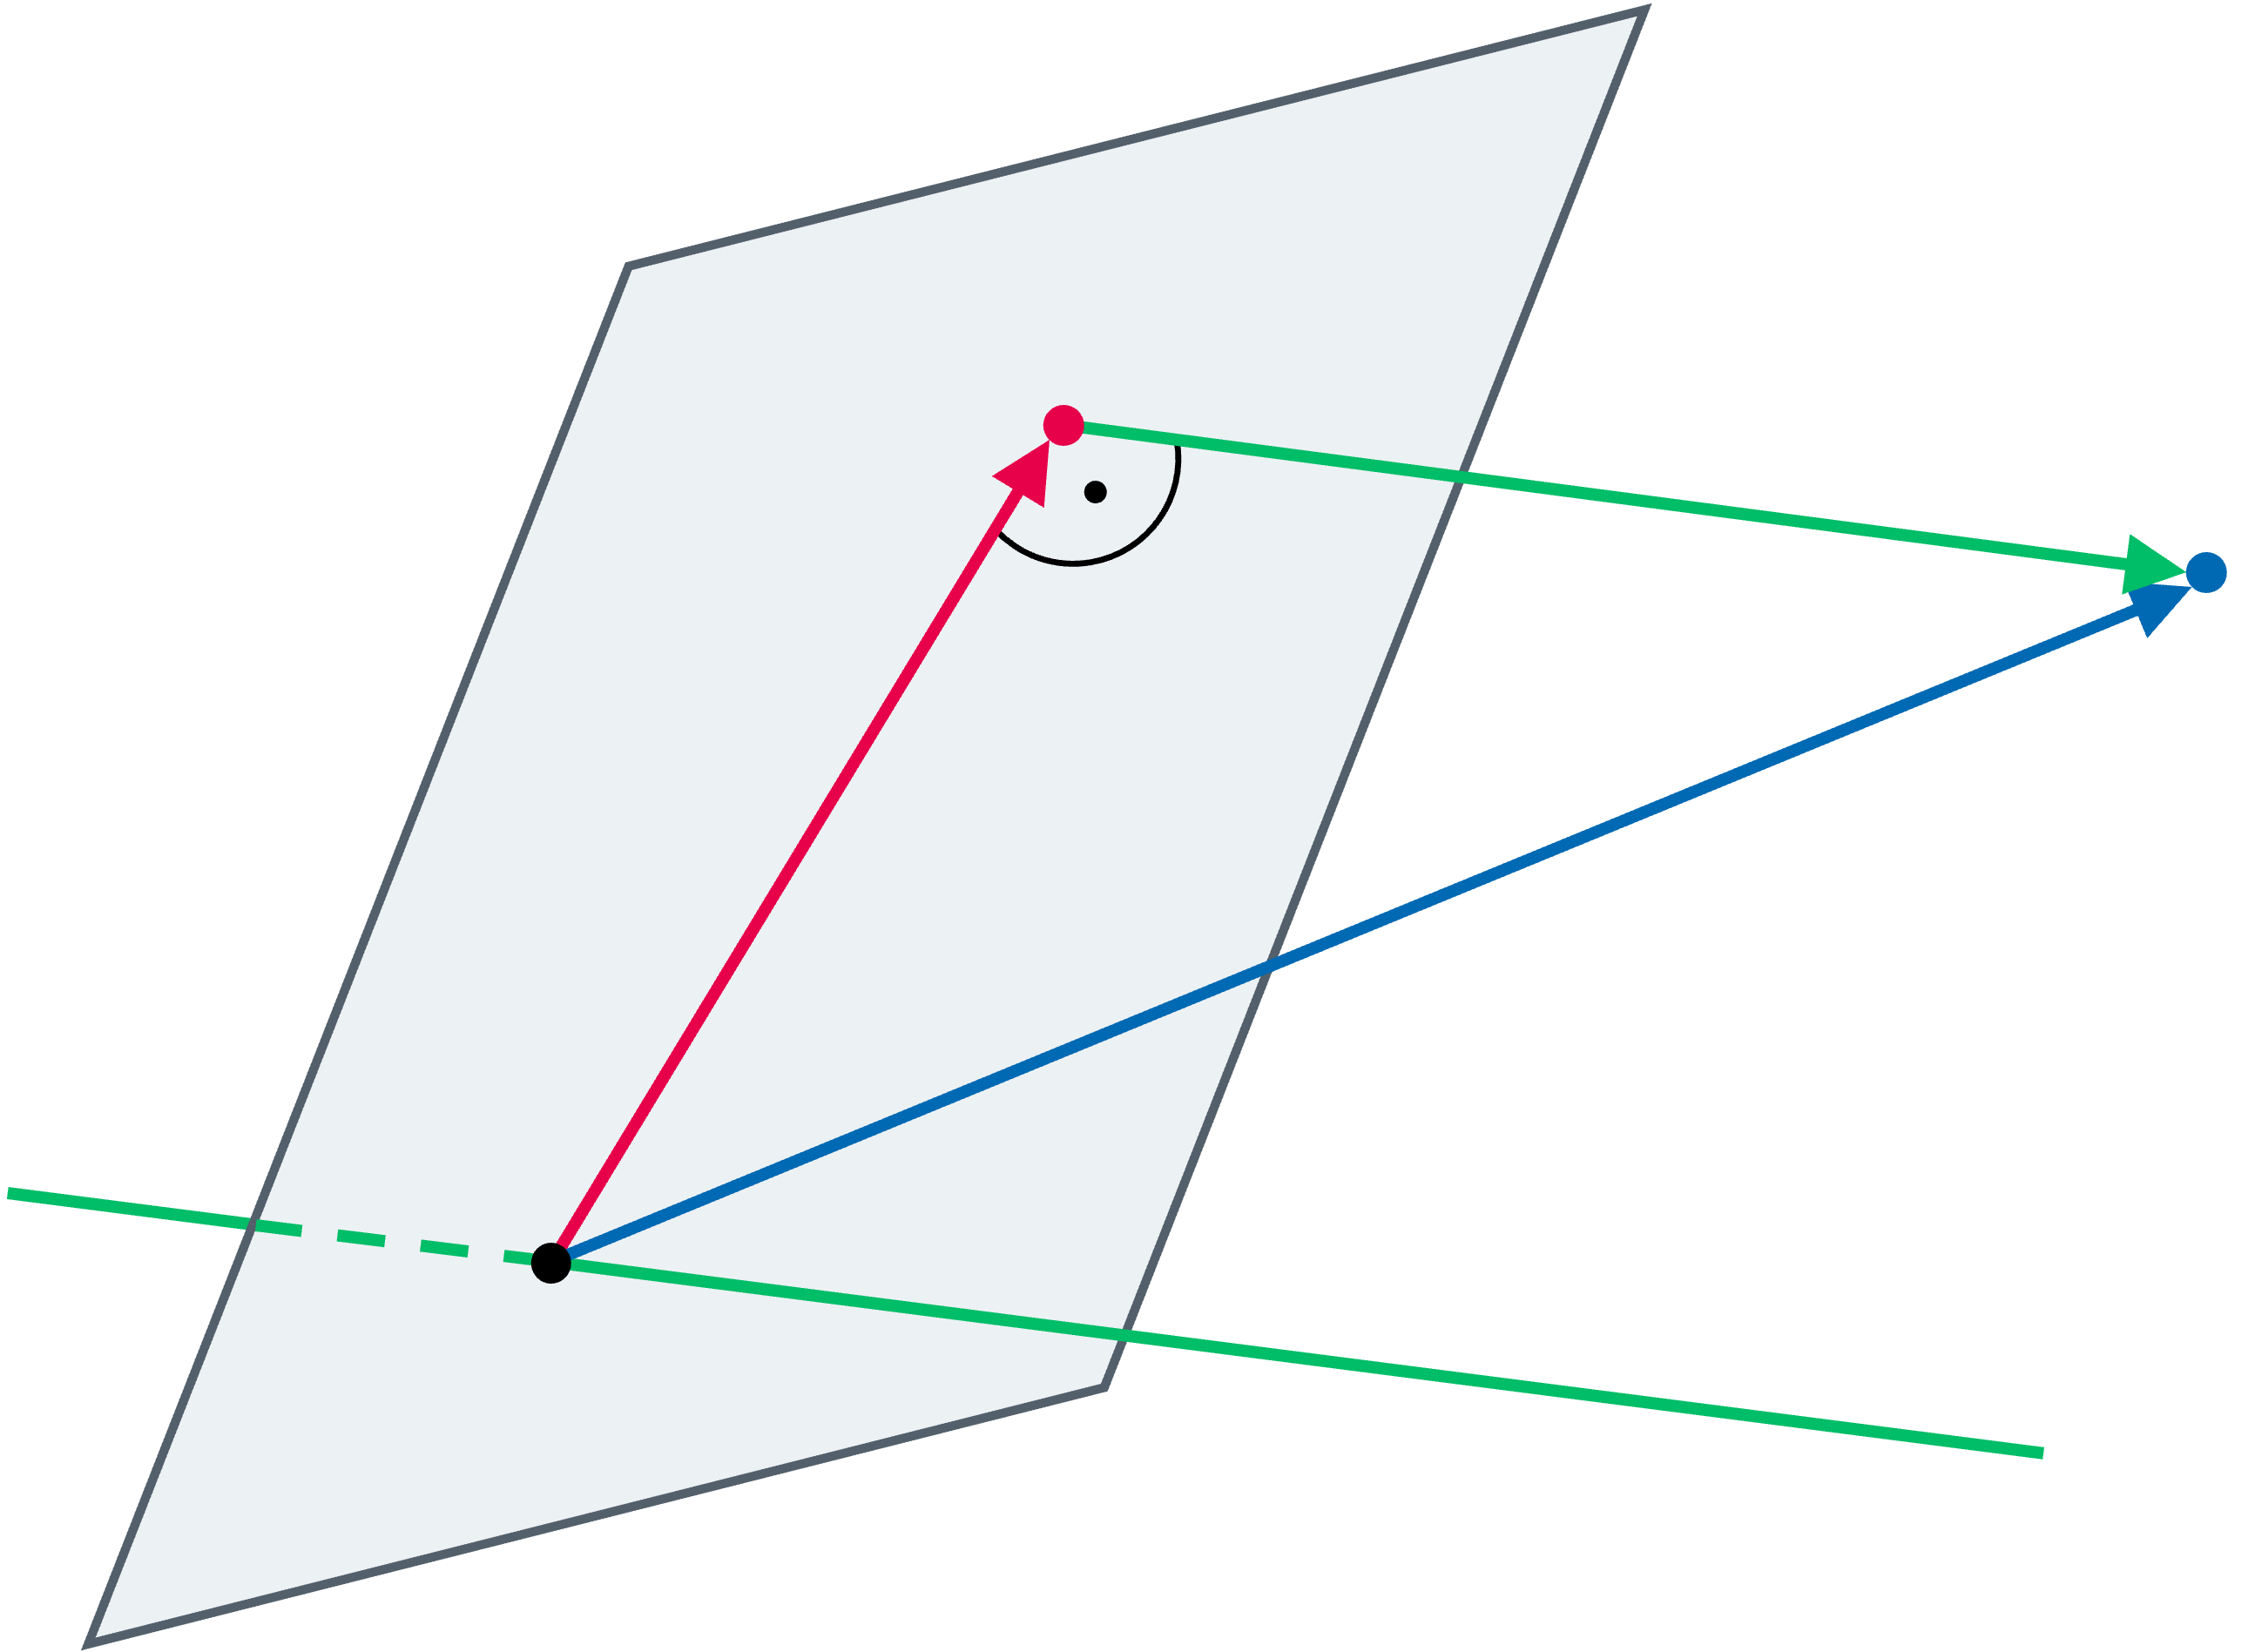
\includegraphics[width=6cm]{other/orthogonal-decomposition}
        };

        % Create scope with normalized axes
        \begin{scope}[
            x={(image.south east)},
            y={(image.north west)}]
         
            % Grid to properly align annotations
            % \draw[help lines, step=0.1] (image.south west) grid ($(image.north east) + (0.001,0)$);

            % Annotate image
            \node[] at (0.22,0.18) {$\mathbf{0}$};
            \node[] at (0.35,0.60) {\color{blue} $\mathbf{u}$};
            \node[] at (0.80,0.45) {\color{red} $\mathbf{v}$};
            \node[] at (0.20,0.75) {\color{blue} $U$};
            \node[] at (0.75,0.08) {\color{pptx-green} $U^{\bot}$};
            \node[] at (0.80,0.75) {${\color{red} \mathbf{v}} - {\color{blue}\mathbf{u}}$};
        \end{scope}
    \end{tikzpicture}
    \caption{%
         The orthogonal projection ${\color{blue}\mathbf{u}} = P({\color{red}\mathbf{v}})$ of a vector ${\color{red}\mathbf{v}}$ onto the subspace ${\color{blue}U}$. Note that the vector difference ${\color{red}\mathbf{v}} - {\color{blue}\mathbf{u}}$ is orthogonal to the subspace ${\color{blue}U}$, i.e., the vector ${\color{blue}\mathbf{u}}$ is a vector in ${\color{blue}U}$ that minimizes the distance to ${\color{red}\mathbf{v}}$.
    }
    \label{fig: orthogonal projection}
\end{figure}

Finally, to tie this in with our discussion of conditional expectation, we have to review some (very fundamental) functional analysis as well. For a probability space $(\Omega, \mathcal{A}, \P)$, and $p > 0$, we denote\footnote{Note that $\mathcal{L}^p$ critically depends on the $\sigma$-algebra $\mathcal{A}$ (measurability) and the probability measure $\P$ (integrability), we only drop these in the notation for convenience!} the set of measurable functions $f$ for which $\abs{f}^p$ is integrable with respect to $\P$ by $\mathcal{L}^p$, i.e.,
\[
    \highlightMath{
        \mathcal{L}^p = \set{ f \colon \Omega \to \R \with[\Big] f \text{ is measurable, } \int_{\Omega} \abs{f(\omega)}^p \, \mathrm{d}\P(\omega) < \infty}, \quad p > 0.
    }
\]
On $\mathcal{L}^p$, we can define a seminorm via
\[
    \highlightMath{
        \norm{f}_p = \left( \int_{\Omega} \abs{f(\omega)}^p \, \mathrm{d}\P(\omega) \right)^{\nicefrac{1}{p}}, \quad f \in \mathcal{L}^p.
    }
\]
This does \emph{not} yield a (\qq{true}) norm since any two functions $f$ and $g$ that agree almost surely (but may differ on a null set) will share the same seminorm, i.e. $\norm{f}_p = \norm{g}_p$. In particular, $\norm{f}_p = 0$ does \emph{not} imply $f = 0$ (but only $f = 0$ almost surely). However, this can easily be fixed by considering the set $L^p$ of equivalence classes
\[
    [f] = \set{g \in \mathcal{L}^p \with f \sim g},
\]
where
\[
    f \sim g \text{ if and only if } f - g = 0 \text{ almost surely,}
\]
i.e., we simply identify all functions that agree almost surely. On $L^p = \mathcal{L}^p /{\sim}$, we define $\norm{[f]}_p = \norm{f}_p$, and one can check that this indeed defines a norm on $L^p$, turning the latter into a \emph{normed space}. Moreover, one can show (cf. \href{https://en.wikipedia.org/wiki/Riesz–Fischer_theorem#Completeness_of_Lp,_0_%3C_p_≤_∞}{Riesz–Fischer theorem}) that the $L^p$-spaces are \emph{complete} (i.e., every Cauchy sequence converges) with respect to this norm and hence, are \emph{Banach spaces}.

Among all $L^p$-spaces, the space $L^2$ of (equivalence classes of) square-integrable functions is special, as it is the only $L^p$-space that can be equipped with an inner product that induces the norm $\norm{\cdot}_2$ we defined earlier (i.e., $L^2$ is a \emph{Hilbert space}). Indeed, for functions\footnote{For convenience, from now on we will simply speak of functions instead of equivalence classes of functions, and we will also drop the brackets for the equivalence classes.} $f, g \in L^2$, defining
\[
    \highlightMath{
        \langle f, g \rangle_2 = \int_{\Omega} f(\omega) g(\omega) \, \mathrm{d}\P(\omega)
    }
\]
yields an inner product on $L^2$ satisfying $\langle f, f \rangle_2 = \norm{f}^2_2$. Using these newly introduced concepts, the property \eqref{eq: orthogonality of conditional expectation} of the conditional expectation $\Ex{Y \given X}$ can be reformulated as
\[
    \langle Z, Y - \Ex{Y \given X} \rangle_2 = 0,
\]
i.e., the difference between $Y$ and the conditional expectation $\Ex{Y \given X}$ is orthogonal to every $\sigma(X)$-measurable, integrable random variable $Z$. Moreover, note that the space of $\sigma(X)$-measurable, square-integrable random variables is a subspace of all square-integrable random variables on $(\Omega, \mathcal{A}, \P)$. Since the conditional expectation $\Ex{Y \given X}$ is, by definition, also $\sigma(X)$-measurable, identity \eqref{eq: orthogonality of conditional expectation} thus implies that the conditional expectation of $Y$ given $X$ is the orthogonal projection of $Y$ onto the subspace of $\sigma(X)$-measurable, square-integrable random variables on $(\Omega, \mathcal{A}, \P)$. As discussed earlier, this also implies that $\Ex{Y \given X}$ is the random variable in the space of $\sigma(X)$-measurable, square-integrable random variables that is closest to $Y$ with respect to the norm $\norm{\cdot}_2$. In other words, taking into account all the information provided by the input $X$, the conditional expectation $\Ex{Y \given X}$ is our best guess at the value of the output $Y$.

Finally, note that the conditional expectation $\Ex{Y \given X}$ depends on $X$ only via the $\sigma$-algebra $\sigma(X)$ generated by $X$, and, indeed, it makes perfect sense to define the conditional expectation of $Y$ given a sub-$\sigma$-algebra $\mathcal{F} \subset \mathcal{A}$. Also, one can prove existence of the conditional expectation $\Ex{Y \given \mathcal{F}}$ assuming that $\Ex{\abs{Y}} < \infty$.

To conclude this intermezzo on conditional expectation, we list some\footnote{Note that this is merely a selection. In fact, there are many other useful properties of conditional expectation, such as monotone convergence, dominated convergence, Fatou's lemma, Jensen's inequality, and many more.} important properties\footnote{Again, these identities/inequalities are to be understood in an almost sure sense.} of conditional expectation:
\begin{itemize}
    \label{itm: properties of conditional expectation}
    \item $\Ex{\Ex{Y \given \mathcal{F}}} = \Ex{Y} \quad$ (law of total expectation)

    \item $\Ex{\lambda Y + Z \given \mathcal{F}} = \lambda \Ex{Y \given \mathcal{F}} + \Ex{Z \given \mathcal{F}} \quad$ (linearity)

    \item If $Y \leq Z$, then $\Ex{Y \given \mathcal{F}} \leq \Ex{Z \given \mathcal{F}}\quad$ (monotonicity)

    \item If $Y$ is independent of $\sigma(Z, \mathcal{F})$, then $\Ex{YZ \given \mathcal{F}} = \Ex{Y} \Ex{Z \given \mathcal{F}} \quad$ (pulling out independent factors)
    
    \item In particular, if $Y$ is independent of $\mathcal{F}$, then $\Ex{Y \given \mathcal{F}} = \Ex{Y} \quad$ (pulling out independent factors)

    \item If $Y$ is $\mathcal{F}$-measurable, then $\Ex{Y \given \mathcal{F}} = Y \quad$ (stability)

    \item In particular, for sub-$\sigma$-algebras $\mathcal{F}_1 \subset \mathcal{F}_2 \subset \mathcal{A}$, we have $\Ex{\Ex{ Y \given \mathcal{F}_1} \given \mathcal{F}_2} = \Ex{ Y \given \mathcal{F}_1} \quad$ (stability)

    \item If $Y$ is $\mathcal{F}$-measurable, then $\Ex{YZ \given \mathcal{F}} = Y \Ex{Z \given \mathcal{F}} \quad$ (pulling out known factors)

    \item For sub-$\sigma$-algebras $\mathcal{F}_1 \subset \mathcal{F}_2 \subset \mathcal{A}$, we have $\Ex{\Ex{ Y \given \mathcal{F}_2} \given \mathcal{F}_1} = \Ex{ Y \given \mathcal{F}_1} \quad$ (tower rule)
\end{itemize}

Let us return to our discussion of conditional expectation in the setting of minimizing the mean-squared error $\mathcal{E}_2(f) = \ex{\norm{f(X) - Y}^2}$. First, note that the conditional expectation of $Y \in \R^d$ given $X$ is simply the vector of conditional expectations of $Y_i$ given $X$ for $i = 1, \dots, d$, i.e.,
\[
    \Ex{Y \given X} = \begin{pmatrix}
        \Ex{Y_1 \given X} \\
        \vdots \\
        \Ex{Y_d \given X}
    \end{pmatrix}.
\]
Based on the observation that the conditional expectation minimizes the $L^2$-distance between $Y$ and the space of $\sigma(X)$-measurable, square-integrable random variables, we define
\[
    f_Y \colon \mathcal{X} \to \R^d, \quad f_Y(x) = \Ex{Y \given X = x},
\]
i.e., $f_Y(X) = \Ex{Y \given X}$. We have the following result:
\begin{proposition}
\label{prop: decomposition of mean-squared error}
Let $Y \colon \Omega \to \R^d$ be a random variable such that $\Ex{\abs{Y_i}} < \infty$, $i = 1, \dots, d$, and let $X \colon \Omega \to \mathcal{X}$ be a random variable and $f \colon \mathcal{X} \to \R^d$ be a measurable function such that the mean-squared error $\mathcal{E}_2(f)$ exists. Then,
\[
    \mathcal{E}_2(f) = \mathcal{E}_2(f(X), \Ex{Y \given X}) + \Ex{\sigma_Y^2(X)},
\]
where
\[
    \sigma_Y^2(X) = \ex{\norm{Y - \Ex{Y \given X}}^2 \given X}
\]
is the \emph{conditional variance} of $Y$ given $X$. In particular,
\[
    \mathcal{E}_2(\Ex{Y \given X}) = \Ex{\sigma_Y^2(X)} = \ex{\norm{Y - \Ex{Y \given X}}^2}.
\]
\end{proposition}

\begin{proof}
We have
\begin{align*}
    \mathcal{E}_2(f) &= \ex{\norm{f(X) - Y}^2} = \ex{\norm{(f(X) - f_Y(X)) + (f_Y(X) - Y)}^2} \\
        &= \ex{\norm{f(X) - f_Y(X)}^2} + \ex{\norm{f_Y(X) - Y}^2} + 2 \sum_{i=1}^d \Ex{(f_i(X) - \Ex{Y_i \given X}) (\Ex{Y_i \given X} - Y_i)} \\
        &= \ex{\norm{f(X) - f_Y(X)}^2} + \ex{\ex{\norm{f_Y(X) - Y}^2 \given X}} \\[4pt]
        &= \mathcal{E}_2(f(X), \Ex{Y \given X}) + \Ex{\sigma_Y^2(X)},
\end{align*}
where the second-to-last identity follows from the fact that the terms $\Ex{(f_i(X) - \Ex{Y_i \given X}) (\Ex{Y_i \given X} - Y_i)}$ vanish\footnote{Proving this is left as an exercise.} for $i = 1, \dots, d$ and the law of total expectation.
\end{proof}

\begin{remark}
\label{rmk: input-output}
\begin{enumerate}[(i)]
    \item The quantity $\mathcal{E}_2(f(X), \Ex{Y \given X})$ measures the $L^2$-error of using $f(X)$ as an approximation of the conditional expectation $\Ex{Y \given X}$.

    \item The term $\Ex{\sigma_Y^2(X)}$ is independent of the choice of $f \colon \mathcal{X} \to \R^d$. In particular, this shows that the $L^2$-error $\mathcal{E}_2(f)$ is minimized by $f = f_Y = \Ex{Y \given X}$.

    \item The property $\P_{(X, Y)} = \P_{Y \given X} \cdot \P_X$ enables us to consider $\mathcal{X} \times \mathcal{Y}$ sequentially, i.e., as an \emph{input space} $\mathcal{X}$ followed by an \emph{output space} $\mathcal{Y}$, since, for any measurable function $f \colon \mathcal{X} \times \mathcal{Y} \to \R$, we have
        \[
            \Ex{f(X, Y)} = \int_{\mathcal{X}} \left( \int_{\mathcal{Y}} f(x, y) \dP{Y \given X=x}{y} \right) \dP{X}{x}.
        \]
\end{enumerate}
\end{remark}
